\documentclass[a4paper,twocolumn]{article}
\usepackage{graphicx}
\usepackage{listings}
\usepackage[justification=centering]{caption}
\usepackage{subfigure}  
\usepackage{multirow}
\usepackage{balance}
\lstset{language=Matlab}
\lstset{breaklines}
\lstset{extendedchars=false}

\usepackage{amsmath,amsfonts,amsthm,amssymb}
\theoremstyle{definition}
\newtheorem{thm}{Theorem}
\newtheorem{exmp}{Example}
\newtheorem{defn}{Definition}
\newtheorem{lema}{Lemma}
\newtheorem{prop}{Proposition}
\newtheorem{coro}{Corollary}


\renewcommand{\baselinestretch}{1.25}

%------------setlength----------------%
\setlength{\textwidth}{162mm}
%\setlength{\textheight}{190mm}
\setlength{\textheight}{231mm}
\setlength{\headheight}{-0.1cm}
\setlength{\topmargin}{-0.1cm}
\setlength{\oddsidemargin}{-0cm}
\setlength{\evensidemargin}{-0cm}

\setlength\columnsep{12pt}
\setlength\columnseprule{0.4pt}

\setlength{\parskip}{1mm}
\setlength{\unitlength}{1mm}
\setlength{\parindent}{2em}

\title{Project2 - Answers to problems}

\author{Li Zhiqi\quad3180103041}

\begin{document}
\maketitle
\section{Restatement of problems}
The problem to be calculated is the one-dimensional Poisson equation
$$
-u^{\prime \prime}(x)=f(x)
$$
on $\Omega = [0,1]$ with Dirichlet boundary condition. We are supposed to write a  $\mathrm{C}++$ package implementing the multigrid solver to solve it. The package is required to give many options for users to choose from, and we will not list the details here.\\
With the package above, we will answer the following questions:\\\\
(\uppercase\expandafter{\romannumeral2}): For the function
$$
u(x) = \exp(\sin(x)),
$$
derive the corresponding $f(x)$ and the boundary conditions. For $\epsilon = 10^{-8}$ and the zero-vector initial guess, test the multigrid solver for all combinations
of restriction operators, interpolation operators and cycles with $n$ = 128,256,512,1024, report the residual and the reduction rate of the residuals for each V-cycle. Report the maximum norm of the error vector and the corresponding convergence rates.\\\\
(\uppercase\expandafter{\romannumeral3}): Gradually reduce $\epsilon$ towards $2.2\times10^{-16}$ , determine the critical value of $\epsilon$ that the program fail to achieve the preset accuracy. Explain the reason for the failure.\\\\
(\uppercase\expandafter{\romannumeral4}): Design a test with homogeneous boundary conditions and repeat (\uppercase\expandafter{\romannumeral2}).\\\\
The following shows the calculation results of (\uppercase\expandafter{\romannumeral2}), (\uppercase\expandafter{\romannumeral3}) and (\uppercase\expandafter{\romannumeral4}).
You can use the command \textbf{"make run"} to get main results listed below. When running, exit matlab to get the next plot.
\section{Results of (\uppercase\expandafter{\romannumeral2})}
In this section, we will show the format of the input file, display of the solution for different grids , and detailed analysis for each grid.\\
Withoout additional explanation, we set 
$$
f(x) = \sin x e^{\sin x}-\cos^2 xe^{\sin x},
$$
and
$$
u(0) = 1,u(1) = e^{\sin(1)} ,
$$
with the exact solution
$$
u(x) = e^{\sin x}.
$$ 
\subsection{Format of the input file}
In the package, it is necessary to do calculations by writing a input file where the boundary conditions, restriction operators, interpolation operators, cycles, criteria and other information are given.The specific format is as follows:
\setlength{\tabcolsep}{1mm}{
\begin{table}[!htp]
	\footnotesize
	\centering
	\begin{tabular}{|c|c|c|c|}
		\hline	
		Index&boundary&restriction&interpolation\\
		\hline		
		1&nonhomogeneous&injection&quadratic\\	
		\hline		
		2& homogeneous&full\_weighting&linear\\	
		\hline \hline
		cycles&criteria\_type&criteria& initial\_type\\
		\hline
		V\_cycle & 1 &1e-8 & 0 \\
		\hline
		fm\_cycle & 0 &10 & 0 \\
		\hline
		\hline
		n & analysis &&\\
		\hline
		128 & 1 &&\\
		\hline
		1024& 0 &&\\
		\hline
	\end{tabular}
	\caption{Input format}
\end{table}}
\newpage
\noindent the above input format, criteria\_type equals to 1 means we take relative accuracy as  stopping criteria, and in this case criteria is relative accuracy; Criteria\_type equals to 0 means we take the number of maximum iterations as stopping criteria, and in this case criteria is the number of maximum iterations. Initial\_type equals to 1 means we choose  zero-vector as initial guess. Analysis equals to 1 means the program will report the residual and the reduction rate of the residuals for V-cycle, and return the maximum norm of the error vector for both V-cycle and full multigrid cycle, while it will return calculation results and show the effect of results if analysis equals to 0.\\
By the way, the stopping criteria will not work if the cycle is full multigrid cycle. That's because full multigrid cycle scheme is not an iterative method.
\subsection{Display of the solution}
Firstly, we show the calculation effect by several examples. The input file is as follows:
\setlength{\tabcolsep}{1mm}{
	\begin{table}[!htp]
		\footnotesize
		\centering
		\begin{tabular}{|c|c|c|c|}
			\hline	
			Index&boundary&restriction&interpolation\\
			\hline		
			1&nonhomogeneous&injection&quadratic\\	
			\hline		
			2& nonhomogeneous&full\_weighting&linear\\	
			\hline \hline
			cycles&criteria\_type&criteria& initial\_type\\
			\hline
			V\_cycle & 0 &10 & 0 \\
			\hline
			fm\_cycle & 1 &1e-8 & 0 \\
			\hline
			\hline
			n & analysis &&\\
			\hline
			128 & 0 &&\\
			\hline
			1024& 0 &&\\
			\hline
		\end{tabular}
		\caption{Input test2-2}
\end{table}}\\
Use command \textbf{"make test22"} to get following results. Here are plots from the program:
\begin{figure}[!htp]   
	\centering
	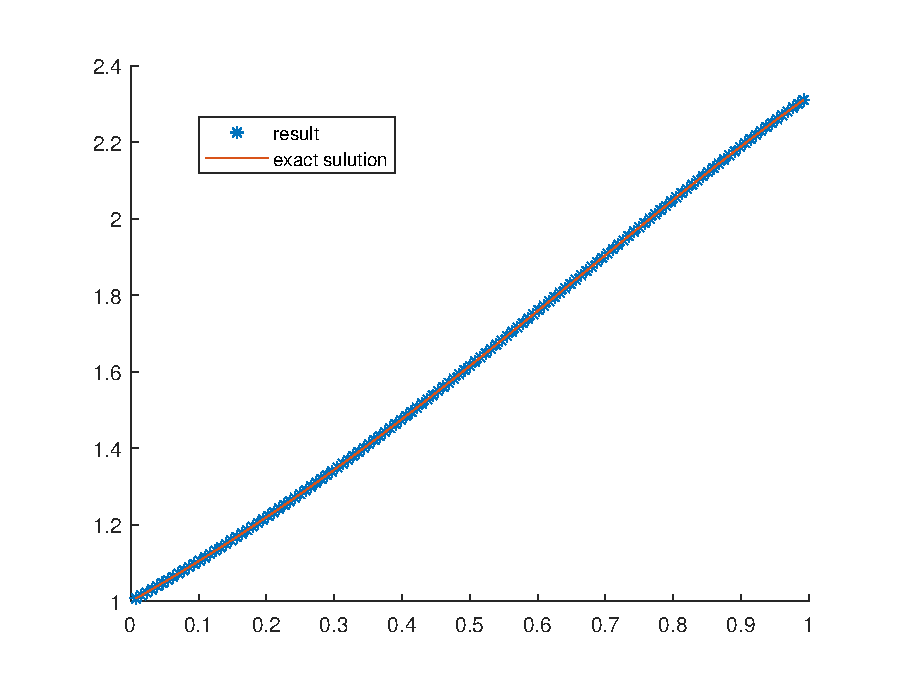
\includegraphics[width=7cm]{Pictures/F22_1.eps}
	\caption{V-cycle, $n = 128$}
\end{figure}
\begin{figure}[!htp]   
	\centering
	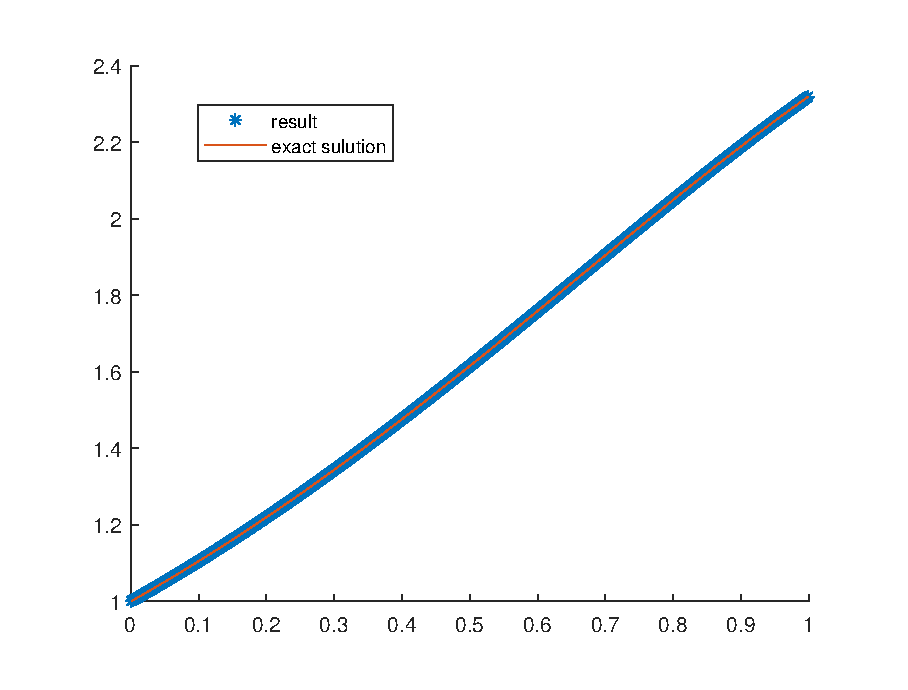
\includegraphics[width=7cm]{Pictures/F22_2.eps}
	\caption{full multigrid cycle, $n = 1024$}
\end{figure}\\
In the figures above, Blue asterisks indicate
results we calculate, while the red line shows the exact solution. Obviously, our program preforms well. You can get the result(a long vector) by reading variable 'result' in the corresponding .m file.
\subsection{Analysis of V-cycle}
In this part, we will test the V-cycle solver for all combinations of restriction operators and interpolation operators with $n$ = 128,256,512,1024. We will report the residual and the reduction rate of the residuals, the maximum norm of the error vector and the corresponding convergence rates.\\
We set the stopping criteria is the relative accuracy and $\epsilon = 10^{-8}$. Take zero-vector  as initial guess.
\subsubsection{Full-weighting and linear interpolation}
Firstly, we use full-weighting and linear interpolation as restriction operator and interpolation operator.The input file is as follows:
\setlength{\tabcolsep}{1mm}{
	\begin{table}[!htp]
		\footnotesize
		\centering
		\begin{tabular}{|c|c|c|c|}
			\hline	
			Index&boundary&restriction&interpolation\\
			\hline		
			1&nonhomogeneous&full\_weighting&linear\\	
			\hline		
			2& nonhomogeneous&full\_weighting&linear\\	
			\hline		
			3& nonhomogeneous&full\_weighting&linear\\
			\hline		
			4& nonhomogeneous&full\_weighting&linear\\
			\hline \hline
			cycles&criteria\_type&criteria& initial\_type\\
			\hline
			V\_cycle & 1 &1e-8 & 0 \\
			\hline
			V\_cycle & 1 &1e-8 & 0 \\
			\hline
			V\_cycle & 1 &1e-8 & 0 \\
			\hline
			V\_cycle & 1 &1e-8 & 0 \\
			\hline
			\hline
			n & analysis &&\\
			\hline
			128 & 1 &&\\
			\hline
			256& 1 &&\\
			\hline
			512& 1 &&\\
			\hline
			1024& 1 &&\\
			\hline
		\end{tabular}
		\caption{Input test2-3-1}
\end{table}}\\
Use command \textbf{"make test231"} to get results. The residual and the maximum norm of the error vector can be obtained by read corresponding output file in folder 'Output'. (Example:output file 'Output/test231\_128' for $n = 128$ ) The reduction rate of the residuals is shown by running the corresponding .m file. (Example:'V\_cycle\_256' for $n = 256$)\\
Below we show the main results.\\
$n=128$: (Read 'Output/test231\_128' for details)
\begin{figure}[!htp]   
	\centering
	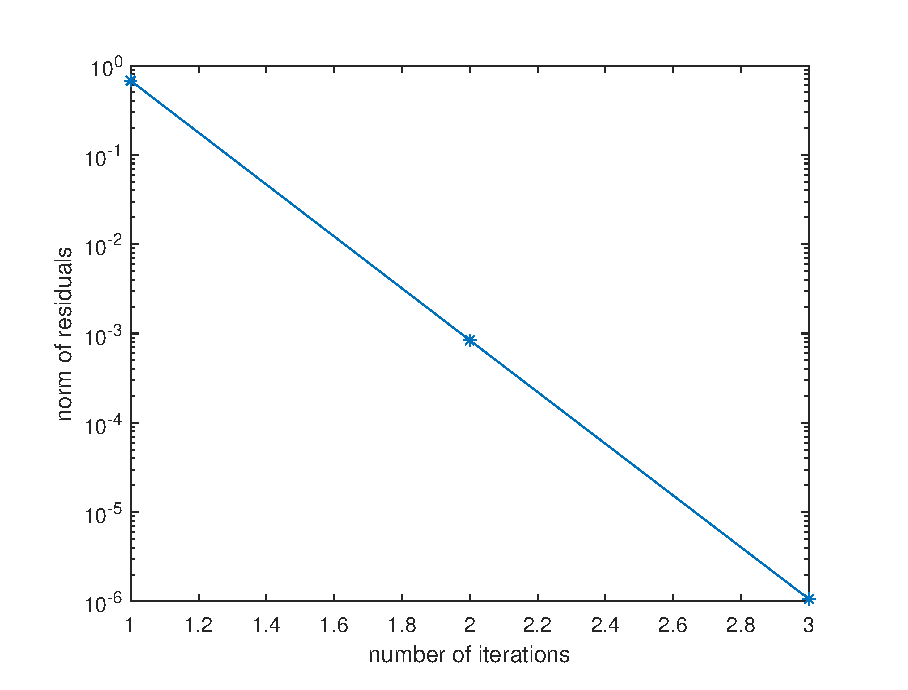
\includegraphics[width=6cm]{Pictures/F231_1.eps}
	\caption{reduction of residuals \\for V-cycle, full-weighting and linear interpolation\\ $n = 128$}
\end{figure}
\newpage
\noindent \emph{Reduction rate of residuals = 0.0012551}\\
\emph{Max\_norm of error vector is 3.09269e-06}\\\\
$n=256$: (Read 'Output/test231\_256' for details)
\begin{figure}[!htp]   
	\centering
	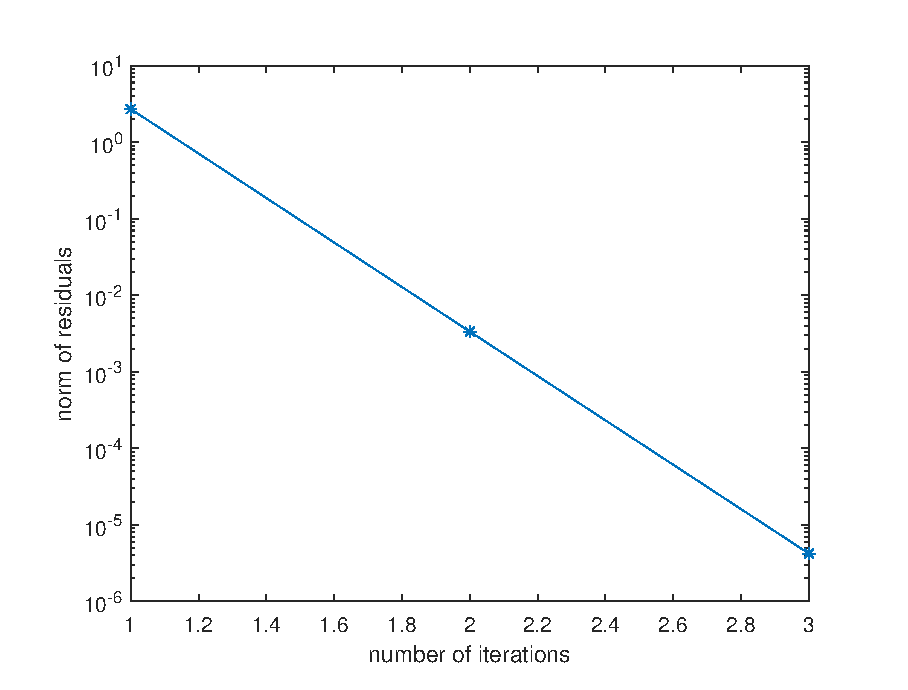
\includegraphics[width=6cm]{Pictures/F231_2.eps}
	\caption{reduction of residuals \\for V-cycle, full-weighting and linear interpolation\\ $n = 256$}
\end{figure}\\
\noindent \emph{Reduction rate of residuals = 0.0012503}\\
\emph{Max\_norm of error vector is 7.74452e-07}\\\\
$n=512$: (Read 'Output/test231\_512' for details)
\begin{figure}[!htp]   
	\centering
	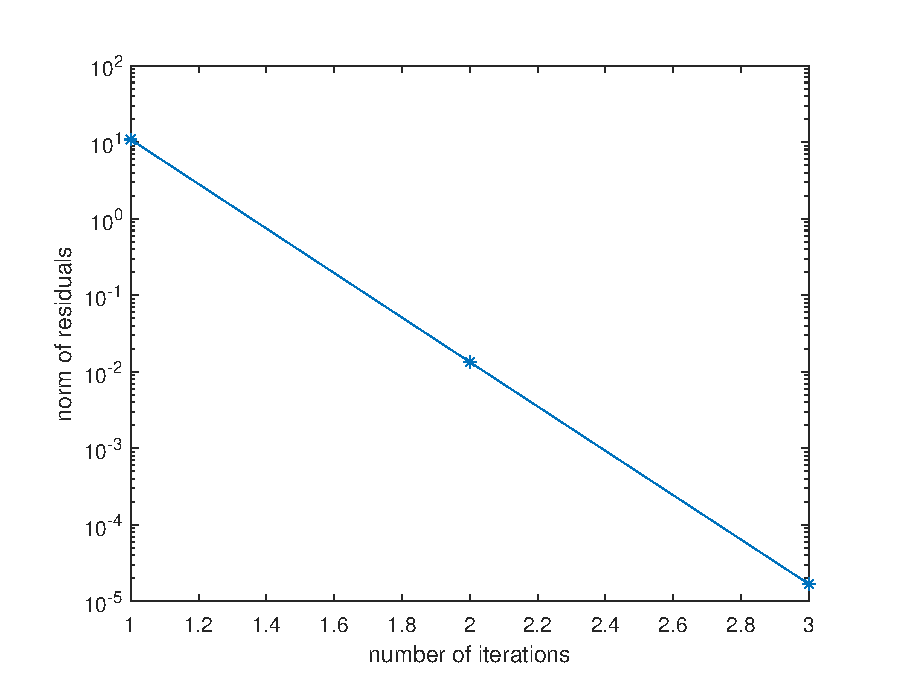
\includegraphics[width=6cm]{Pictures/F231_3.eps}
	\caption{reduction of residuals \\for V-cycle, full-weighting and linear interpolation\\ $n = 512$}
\end{figure}\\
\noindent \emph{Reduction rate of residuals = 0.0012503}\\
\emph{Max\_norm of error vector is 1.94908e-07}\\
\newpage
\noindent $n=1024$: (Read 'Output/test231\_1024' for details)
\begin{figure}[!htp]   
	\centering
	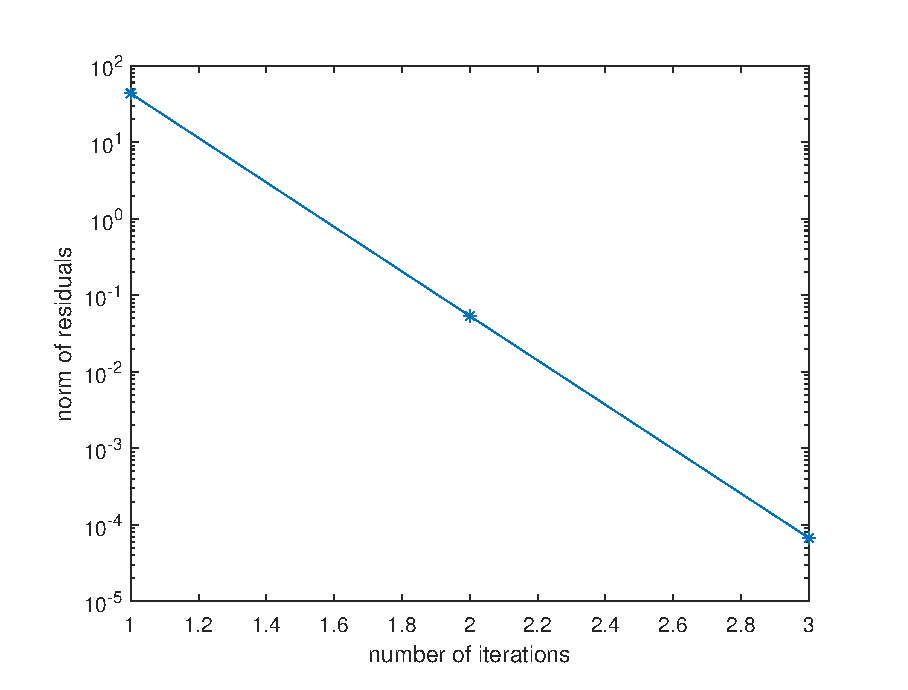
\includegraphics[width=7cm]{Pictures/F231_4.eps}
	\caption{reduction of residuals \\for V-cycle, full-weighting and linear interpolation\\ $n = 1024$}
\end{figure}\\
\noindent \emph{Reduction rate of residuals = 0.0012503}\\
\emph{Max\_norm of error vector is 5.00265e-08}\\\\
Then we have
\begin{table}[!htp]
	\centering
	\begin{tabular}{|c|c|c|}
		\hline	
		n & reduction rate of residuals &max-norm of err  \\
		\hline		
		128 &0.0012551& $3.09269\times 10^{-6}$ \\
		\hline		
		256 &0.0012503& $7.74452\times 10^{-7}$ \\
		\hline		
		512 &0.0012503& $1.94908\times 10^{-7}$ \\
		\hline		
		1024 &0.0012503& $5.00265\times 10^{-8}$ \\
		\hline
	\end{tabular}
	\caption{reduction rate of residuals and maximum norms of error vectors \\for V-cycle, full-weighting and linear interpolation}
\end{table}\\
By simple calculation, we get that the convergence order in this case is 1.9833.
\subsubsection{Full-weighting and quadratic interpolation}
We discuss full-weighting and quadratic interpolation as restriction operator and interpolation operator in this part.  Except for restriction operators and interpolation operators, the inputfile is the same as the previous section. For the whole process is the same as the previous section, we show results only. \\
Use command \textbf{"make test232"} to get results. \\\\
$n=128$: (Read 'Output/test232\_128' for details)
\begin{figure}[!htp]   
	\centering
	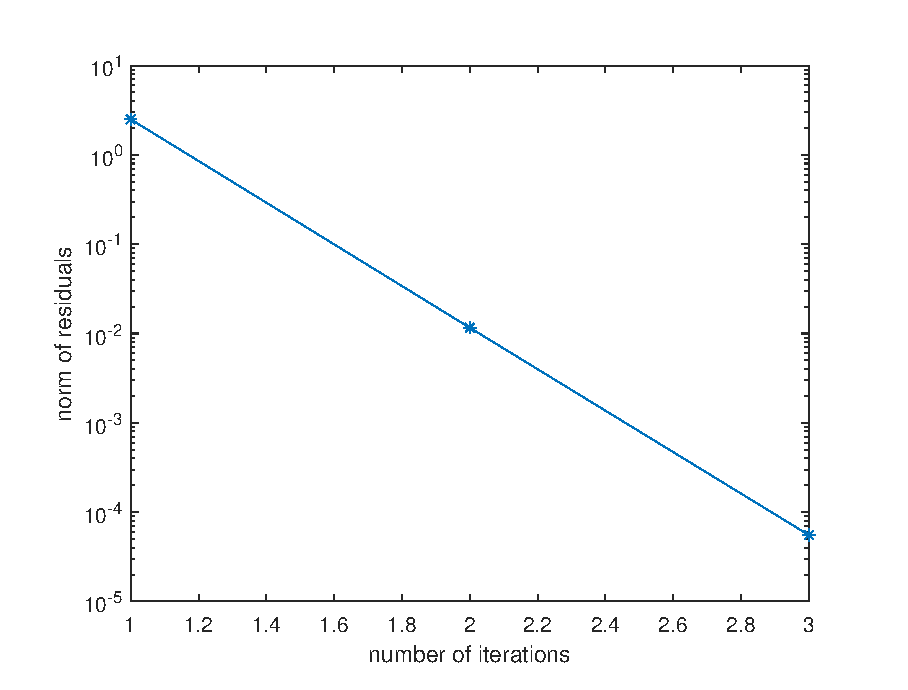
\includegraphics[width=7cm]{Pictures/F232_1.eps}
	\caption{reduction of residuals \\for V-cycle, full-weighting and quadratic interpolation\\ $n = 128$}
\end{figure}\\
\emph{Reduction rate of residuals = 0.0047092}\\
\emph{Max\_norm of error vector is 3.194e-06}\\\\
$n=256$: (Read 'Output/test232\_256' for details)
\begin{figure}[!htp]   
	\centering
	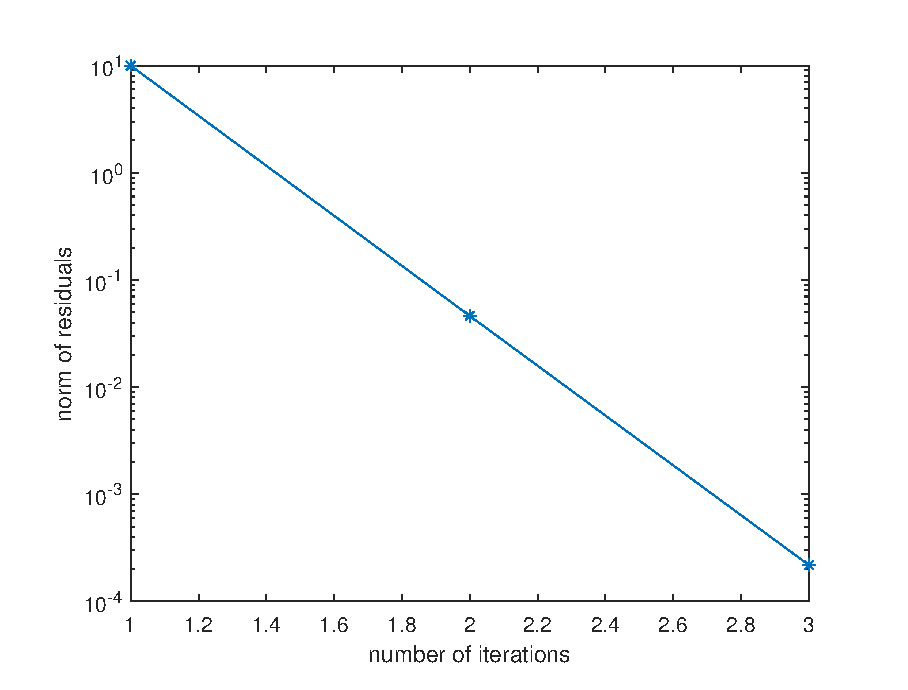
\includegraphics[width=7cm]{Pictures/F232_2.eps}
	\caption{reduction of residuals \\for V-cycle, full-weighting and quadratic interpolation\\ $n = 256$}
\end{figure}\\
\emph{Reduction rate of residuals = 0.0046832}\\
\emph{Max\_norm of error vector is 8.72917e-07}
\newpage
\noindent $n=512$: (Read 'Output/test232\_512' for details)
\begin{figure}[!htp]   
	\centering
	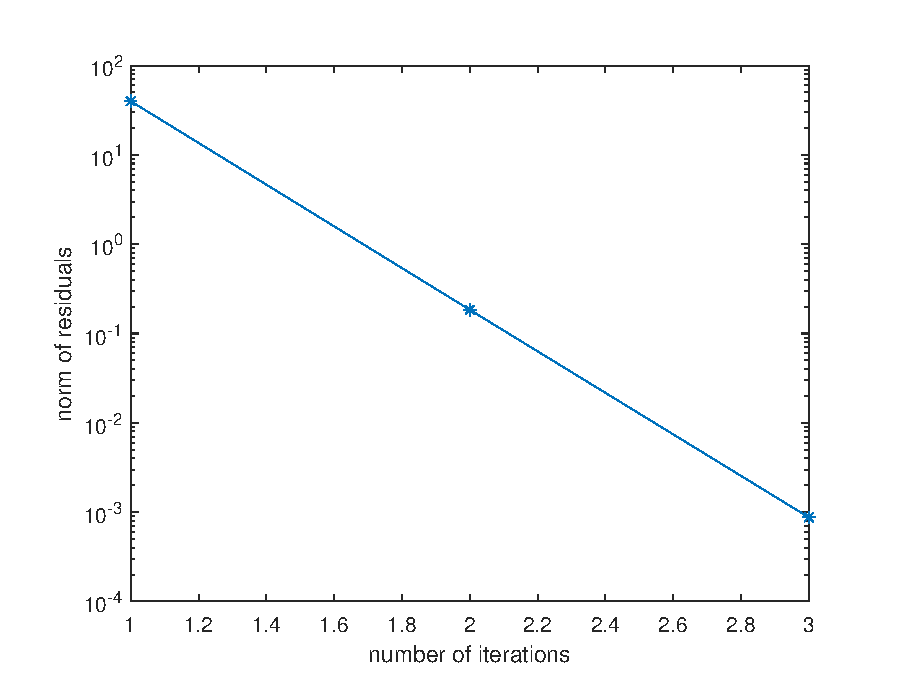
\includegraphics[width=7cm]{Pictures/F232_3.eps}
	\caption{reduction of residuals \\for V-cycle, full-weighting and quadratic interpolation\\ $n = 512$}
\end{figure}\\
\emph{Reduction rate of residuals = 0.0046808}\\
\emph{Max\_norm of error vector is 2.939e-07}\\\\
$n=1024$: (Read 'Output/test232\_1024' for details)
\begin{figure}[!htp]   
	\centering
	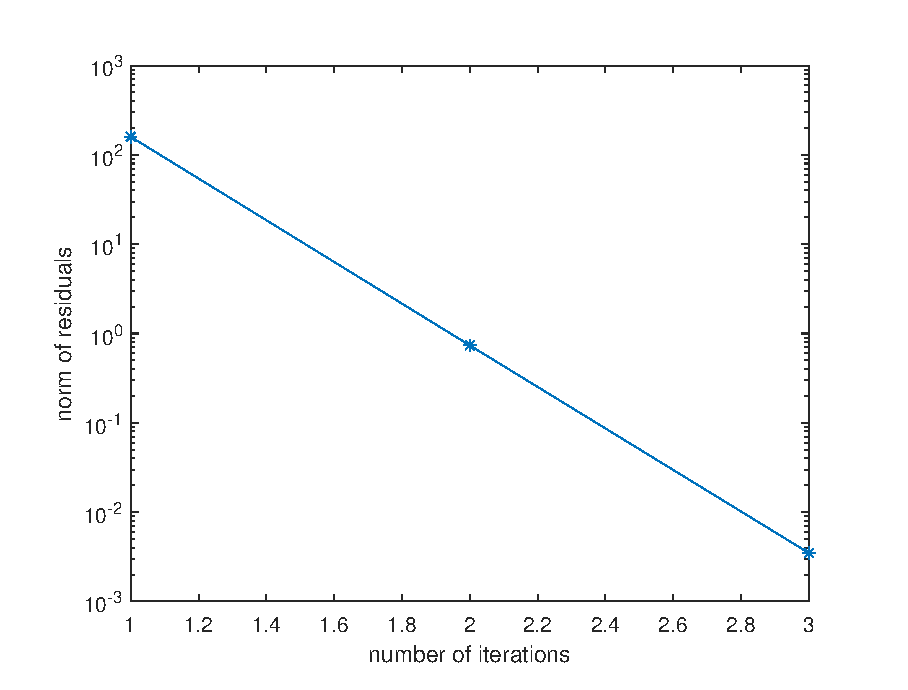
\includegraphics[width=7cm]{Pictures/F232_4.eps}
	\caption{reduction of residuals \\for V-cycle, full-weighting and quadratic interpolation\\ $n = 1024$}
\end{figure}\\
\emph{Reduction rate of residuals = 0.0046798}\\
\emph{Max\_norm of error vector is 1.60175e-07}
\newpage
\noindent Then we have
\begin{table}[!htp]
	\centering
	\begin{tabular}{|c|c|c|}
		\hline	
		n & reduction rate of residuals & max-norm of err  \\
		\hline		
		128 &0.0047092 & $3.194\times 10^{-6}$ \\
		\hline		
		256 &0.0046832 & $8.72917\times 10^{-7}$ \\
		\hline		
		512 &0.0046808 & $2.939\times 10^{-7}$ \\
		\hline		
		1024 &0.0046798 & $1.60175\times 10^{-7}$ \\
		\hline
	\end{tabular}
	\caption{reduction rate of residuals and maximum norms of error vectors \\for V-cycle, full-weighting and quadratic interpolation}
\end{table}\\
The convergence order in this case is 1.4324.
\subsubsection{Injection and linear interpolation}
Take injection and linear interpolation as restriction operator and interpolation operator, and the rest of the input files remain the same. To avoid meaningless repetition, we only show the reduction rate of the residuals and the maximum norm of the error vector for different $n$ in the form of a table. More details can be obtained by reading corresponding output files.\\
Use command \textbf{"make test233"} to get results. \\
\begin{table}[!htp]
	\centering
	\begin{tabular}{|c|c|c|}
		\hline	
		n &reduction rate of residuals & max-norm of err \\
		\hline		
		128 &No data& $3.09088\times 10^{-6}$ \\
		\hline		
		256 &No data& $7.72706\times 10^{-7}$ \\
		\hline		
		512 &No data& $1.93176\times 10^{-7}$ \\
		\hline		
		1024 &No data& $4.82939\times 10^{-8}$ \\
		\hline
	\end{tabular}
	\caption{reduction rate of residuals and maximum norms of error vectors \\for V-cycle, injection and linear interpolation}
\end{table}\\
The convergence order in this case is 2.00001.\\\\
\textbf{Explanation for 'No data' in the table}: The program only take one time V-cycle iteration to achieve the preset accuracy, so there is not enough data to calculate the reduction rate of residuals.
\newpage
\subsubsection{Injection and quadratic interpolation}
In the last part, we take injection and quadratic interpolation as restriction operator and interpolation operator. Main results are shown as follows. More details can be obtained by reading corresponding output files.\\
Use command \textbf{"make test234"} to get results.\\
\begin{table}[!htp]
	\centering
	\begin{tabular}{|c|c|c|}
		\hline	
		n &reduction rate of residuals & max-norm of err \\
		\hline		
		128 &0.0034686& $3.13299\times 10^{-6}$ \\
		\hline		
		256 &0.0034472& $8.13514\times 10^{-7}$ \\
		\hline		
		512 &0.0034449& $2.33956\times 10^{-7}$ \\
		\hline		
		1024 &0.003444& $8.97677\times 10^{-8}$ \\
		\hline
	\end{tabular}
	\caption{reduction rate of residuals and maximum norms of error vectors \\for V-cycle, injection and quadratic interpolation}
\end{table}\\
The convergence order in this case is 1.69078.
\subsection{Analysis of full multigrid cycle}
In this part, we will test the full multigrid cycle solver for all combinations of restriction operators and interpolation operators with $n$ = 128,256,512,1024. We will report the maximum norm of the error vector and the corresponding convergence rates.
\subsubsection{Full-weighting and linear interpolation}
Similar to the case of V-cycle, the input file is as follows:
\setlength{\tabcolsep}{1mm}{
	\begin{table}[!htp]
		\footnotesize
		\centering
		\begin{tabular}{|c|c|c|c|}
			\hline	
			Index&boundary&restriction&interpolation\\
			\hline		
			1&nonhomogeneous&full\_weighting&linear\\	
			\hline		
			2& nonhomogeneous&full\_weighting&linear\\	
			\hline		
			3& nonhomogeneous&full\_weighting&linear\\
			\hline		
			4& nonhomogeneous&full\_weighting&linear\\
			\hline \hline
			cycles&criteria\_type&criteria& initial\_type\\
			\hline
			fm\_cycle & 1 &1e-8 & 0 \\
			\hline
			fm\_cycle & 1 &1e-8 & 0 \\
			\hline
			fm\_cycle & 1 &1e-8 & 0 \\
			\hline
			fm\_cycle & 1 &1e-8 & 0 \\
			\hline
			\hline
			n & analysis &&\\
			\hline
			128 & 1 &&\\
			\hline
			256& 1 &&\\
			\hline
			512& 1 &&\\
			\hline
			1024& 1 &&\\
			\hline
		\end{tabular}
		\caption{Input test2-4-1}
\end{table}}
\newpage
\noindent Use command \textbf{"make test241"} to get results. 
\begin{table}[!htp]
	\centering
	\begin{tabular}{|c|c|}
		\hline	
		n  & max-norm of err \\
		\hline		
		128 & $3.13706\times 10^{-6}$ \\
		\hline		
		256 & $7.66122\times 10^{-7}$ \\
		\hline		
		512 & $1.92771\times 10^{-7}$ \\
		\hline		
		1024 & $5.60661\times 10^{-8}$ \\
		\hline
	\end{tabular}
	\caption{maximum norms of error vectors \\for full multigrid cycle, full-weighting and linear interpolation}
\end{table}\\
The convergence order in this case is 1.93217.
\subsubsection{Full-weighting and quadratic interpolation}
Except for restriction operators and interpolation operators, the inputfile is the same as the previous section. Similarly, we show results directly: (Use command \textbf{"make test242"} to get results.)
\newpage
\begin{table}[!htp]
	\centering
	\begin{tabular}{|c|c|}
		\hline	
		n  & max-norm of err \\
		\hline		
		128 & $3.48094\times 10^{-6}$ \\
		\hline		
		256 & $8.38495\times 10^{-7}$ \\
		\hline		
		512 & $4.68295\times 10^{-7}$ \\
		\hline		
		1024 & $4.27091\times 10^{-7}$ \\
		\hline
	\end{tabular}
	\caption{maximum norms of error vectors \\for full multigrid cycle, full-weighting and quadratic interpolation}
\end{table}
\noindent The convergence order in this case is 1.27108.
\subsubsection{Injection and linear interpolation}
Show results directly: (Use command \textbf{"make test243"} to get results.)
\begin{table}[!htp]
	\centering
	\begin{tabular}{|c|c|}
		\hline	
		n  & max-norm of err \\
		\hline		
		128 & $3.09088\times 10^{-6}$ \\
		\hline		
		256 & $7.72707\times 10^{-7}$ \\
		\hline		
		512 & $1.93176\times 10^{-7}$ \\
		\hline		
		1024 & $4.82939\times 10^{-8}$ \\
		\hline
	\end{tabular}
	\caption{maximum norms of error vectors \\for full multigrid cycle, injection and linear interpolation}
\end{table}\\
The convergence order in this case is 2.00001.
\subsubsection{Injection and quadratic interpolation}
Show results directly: (Use command \textbf{"make test244"} to get results.)
\begin{table}[!htp]
	\centering
	\begin{tabular}{|c|c|}
		\hline	
		n  & max-norm of err \\
		\hline		
		128 & $3.25758\times 10^{-6}$ \\
		\hline		
		256 & $9.10094\times 10^{-7}$ \\
		\hline		
		512 & $3.42653\times 10^{-7}$ \\
		\hline		
		1024 & $2.2947\times 10^{-7}$ \\
		\hline
	\end{tabular}
	\caption{maximum norms of error vectors \\for full multigrid cycle, injection and quadratic interpolation}
\end{table}\\
The convergence order in this case is 1.37377.
\section{Results of (\uppercase\expandafter{\romannumeral3})}
In this section, we will gradually reduce $\epsilon$ towards $2.2\times10^{-16}$ and determine the critical value of $\epsilon$ that the program fail to achieve the preset accuracy. For the reason that full multigrid cycle scheme is not an iterative method, we only consider V-cycle.\\
We use the function and condition in (\uppercase\expandafter{\romannumeral2}), and take $n = 1024$. With different combinations of restriction operators and interpolation operators, we take input file as follows: 
\setlength{\tabcolsep}{1mm}{
	\begin{table}[!htp]
		\footnotesize
		\centering
		\begin{tabular}{|c|c|c|c|}
			\hline	
			Index&boundary&restriction&interpolation\\
			\hline		
			1&nonhomogeneous&full\_weighting&linear\\	
			\hline		
			2& nonhomogeneous&full\_weighting&quadratic\\	
			\hline		
			3& nonhomogeneous&injection&linear\\
			\hline		
			4& nonhomogeneous&injection&quadratic\\
			\hline \hline
			cycles&criteria\_type&criteria& initial\_type\\
			\hline
			V\_cycle & 0 &10 & 0 \\
			\hline
			V\_cycle & 0 &10 & 0 \\
			\hline
			V\_cycle & 0 &10 & 0 \\
			\hline
			V\_cycle & 0 &10 & 0 \\
			\hline
			\hline
			n & analysis &&\\
			\hline
			1024 & 1 &&\\
			\hline
			1024& 1 &&\\
			\hline
			1024& 1 &&\\
			\hline
			1024& 1 &&\\
			\hline
		\end{tabular}
		\caption{Input test3}
\end{table}}\\
the result is as follows: (Use command \textbf{"make test3"} to get results.)\\
Full-weighting and linear interpolation:
\begin{figure}[!htp]   
	\centering
	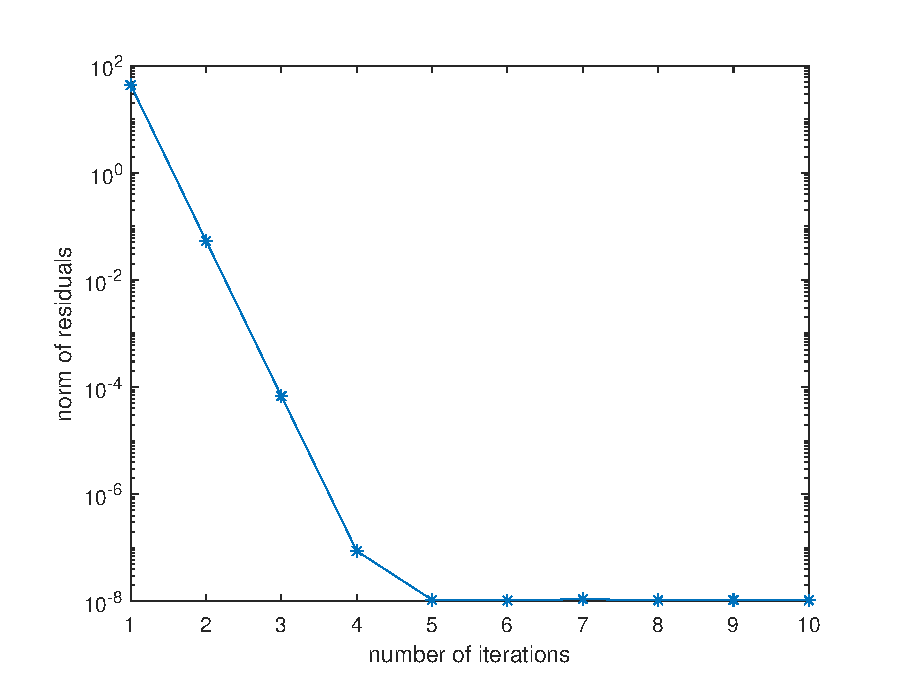
\includegraphics[width=6cm]{Pictures/F3_1.eps}
	\caption{norm of residuals \\for V-cycle, full-weighting and linear interpolation\\ $n = 1024$}
\end{figure}\\
Then we get relative accuracy 
$$
\epsilon = \left \| \textbf{r} \right \| / \left \| \textbf{f} \right \| = 3.94737\times10^{-15} \ ,
$$ 
where $\left \| \textbf{r} \right \| $ is the smallest norm of residual that can be achieved in iteration. \\
Similarly, we get
\begin{table}[!htp]
	\centering
	\begin{tabular}{|c|c|c|}
		\hline	
		restriction&interpolationn  & $\epsilon$ \\
		\hline		
		full\_weighting&linear & $3.94737\times10^{-15}$ \\
		\hline		
		full\_weighting&quadratic & $3.78708\times 10^{-15}$ \\
		\hline		
		injection &linear& $4.46420\times 10^{-15}$ \\
		\hline		
		injection&quadratic & $4.45193\times 10^{-15}$ \\
		\hline
	\end{tabular}
	\caption{relative accuracy $\epsilon$ \\that program fail to achieve\\for V-cycle, $n = 1024$}
\end{table}\\
The main reason for the failure is the restriction of double and the accumulation of round-off errors. The restriction and interpolation of vectors between grids and iteratively solving linear systems both cause round-off errors.
\section{Results of (\uppercase\expandafter{\romannumeral4})}
Firstly we list the function and conditions of the test.
We set 
$$
f(x) = \pi^2\sin \pi x 
$$
on $\Omega = [0,1]$ with homogeneous condition
$$
u(0) = 0,u(1) = 0 ,
$$
with the exact solution
$$
u(x) = \sin \pi x .
$$ 
Same as question 2, we will show the plots of solution for different grids and detailed analysis for each grid.
\subsection{Display of the solution}
We will show the calculation effect by several examples. The input file is as follows:
\setlength{\tabcolsep}{1mm}{
	\begin{table}[!htp]
		\footnotesize
		\centering
		\begin{tabular}{|c|c|c|c|}
			\hline	
			Index&boundary&restriction&interpolation\\
			\hline		
			1&homogeneous&injection&quadratic\\	
			\hline		
			2&homogeneous&full\_weighting&linear\\	
			\hline \hline
			cycles&criteria\_type&criteria& initial\_type\\
			\hline
			V\_cycle & 0 &10 & 0 \\
			\hline
			fm\_cycle & 1 &1e-8 & 0 \\
			\hline
			\hline
			n & analysis &&\\
			\hline
			128 & 0 &&\\
			\hline
			1024& 0 &&\\
			\hline
		\end{tabular}
		\caption{Input test4-1}
\end{table}}\\
\newpage
Use command \textbf{"make test41"} to get following results. Here are plots from the program:
\begin{figure}[!htp]   
	\centering
	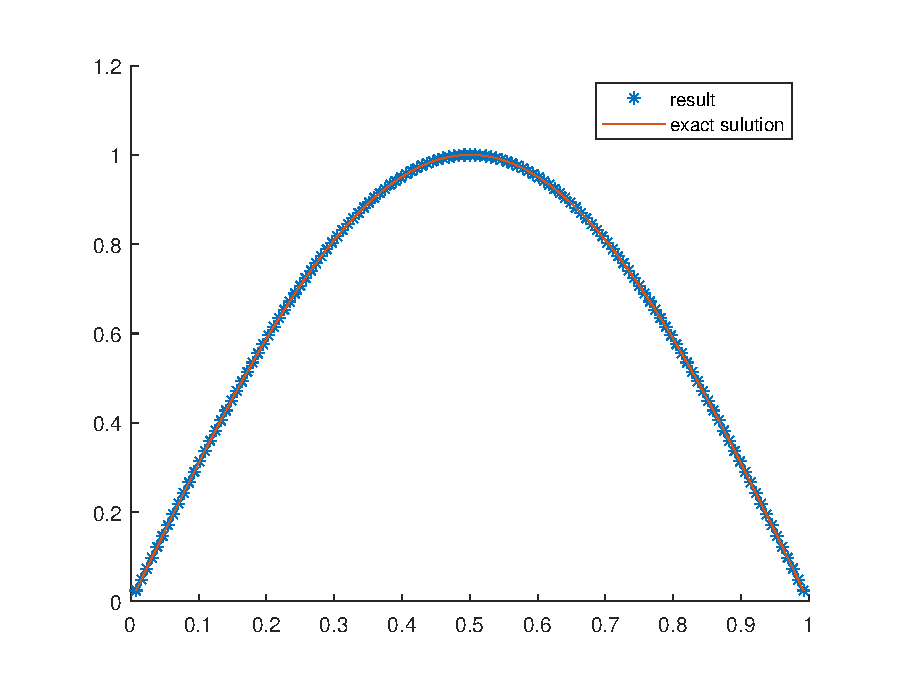
\includegraphics[width=7cm]{Pictures/F41_1.eps}
	\caption{V-cycle, $n = 128$}
\end{figure}
\begin{figure}[!htp]   
	\centering
	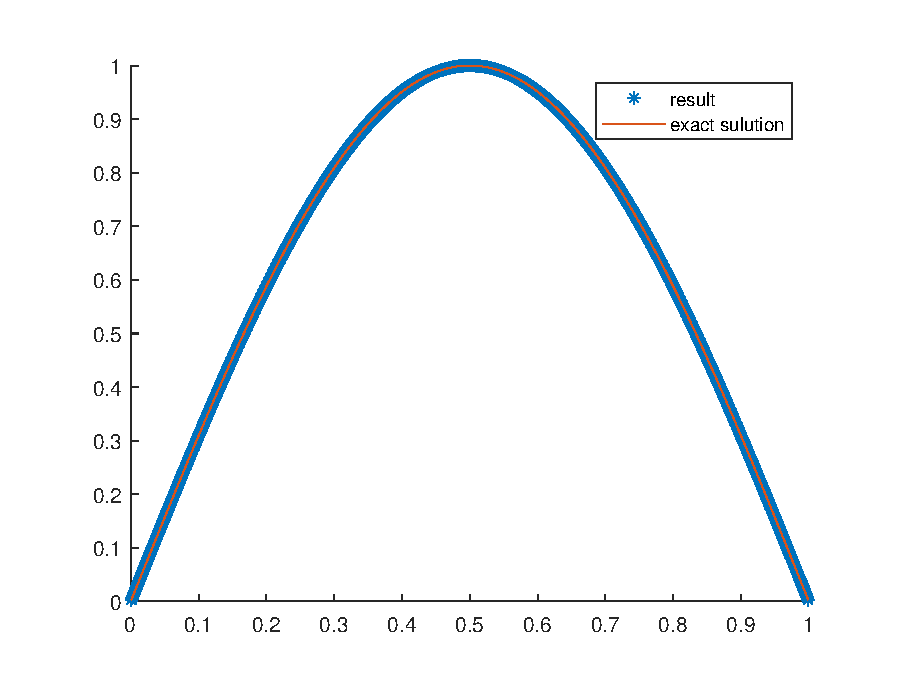
\includegraphics[width=7cm]{Pictures/F41_2.eps}
	\caption{full multigrid cycle, $n = 1024$}
\end{figure}\\
In the figures above, Blue asterisks indicate
results we calculate, while the red line shows the exact solution. Our program preforms well one more time. You can get the result(a long vector) by reading variable 'result' in the corresponding .m file.
\subsection{Analysis of V-cycle}
In this part, we will test the V-cycle solver for all combinations of restriction operators and interpolation operators with $n$ = 128,256,512,1024 for the homogeneous case. We will report the residual and the reduction rate of the residuals, the maximum norm of the error vector and the corresponding convergence rates.\\
We set the stopping criteria is the relative accuracy and $\epsilon = 10^{-8}$. Take zero-vector  as initial guess.
\subsubsection{Full-weighting and linear interpolation}
Firstly, we use full-weighting and linear interpolation as restriction operator and interpolation operator.The input file is as follows:
\setlength{\tabcolsep}{1mm}{
	\begin{table}[!htp]
		\footnotesize
		\centering
		\begin{tabular}{|c|c|c|c|}
			\hline	
			Index&boundary&restriction&interpolation\\
			\hline		
			1&homogeneous&full\_weighting&linear\\	
			\hline		
			2& homogeneous&full\_weighting&linear\\	
			\hline		
			3& homogeneous&full\_weighting&linear\\
			\hline		
			4& homogeneous&full\_weighting&linear\\
			\hline \hline
			cycles&criteria\_type&criteria& initial\_type\\
			\hline
			V\_cycle & 1 &1e-8 & 0 \\
			\hline
			V\_cycle & 1 &1e-8 & 0 \\
			\hline
			V\_cycle & 1 &1e-8 & 0 \\
			\hline
			V\_cycle & 1 &1e-8 & 0 \\
			\hline
			\hline
			n & analysis &&\\
			\hline
			128 & 1 &&\\
			\hline
			256& 1 &&\\
			\hline
			512& 1 &&\\
			\hline
			1024& 1 &&\\
			\hline
		\end{tabular}
		\caption{Input test4-2-1}
\end{table}}\\
Use command \textbf{"make test421"} to get results. The residual and the maximum norm of the error vector can be obtained by read corresponding output file in folder 'Output'. (Example:output file 'Output/test421\_128' for $n = 128$ ) The reduction rate of the residuals is shown by running the corresponding .m file. (Example:'V\_cycle\_256' for $n = 256$)\\
Below we show the main results.\\
\newpage
\noindent $n=128$: (Read 'Output/test421\_128' for details)
\begin{figure}[!htp]   
	\centering
	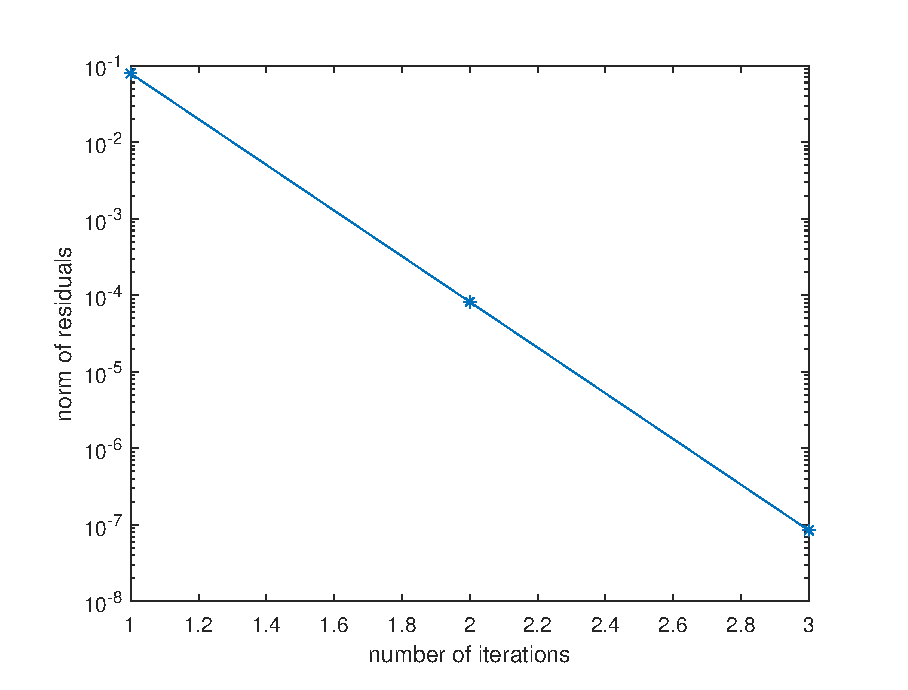
\includegraphics[width=8cm]{Pictures/F421_1.eps}
	\caption{reduction of residuals \\for V-cycle, full-weighting and linear interpolation\\ $n = 128$}
\end{figure}\\
\emph{Reduction rate of residuals = 0.0010379}\\
\emph{Max\_norm of error vector is 5.01998e-05}\\\\
$n=256$: (Read 'Output/test421\_256' for details)
\begin{figure}[!htp]   
	\centering
	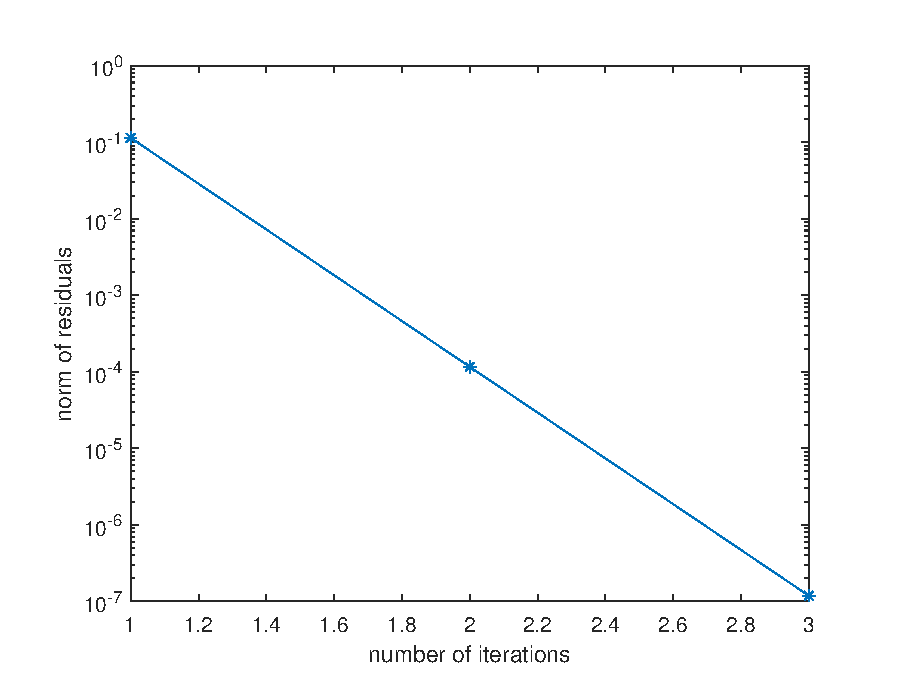
\includegraphics[width=8cm]{Pictures/F421_2.eps}
	\caption{reduction of residuals \\for V-cycle, full-weighting and linear interpolation\\ $n = 256$}
\end{figure}\\
\noindent \emph{Reduction rate of residuals = 0.0010243}\\
\emph{Max\_norm of error vector is 1.25489e-05}\\\\
\newpage
\noindent $n=512$: (Read 'Output/test421\_512' for details)
\begin{figure}[!htp]   
	\centering
	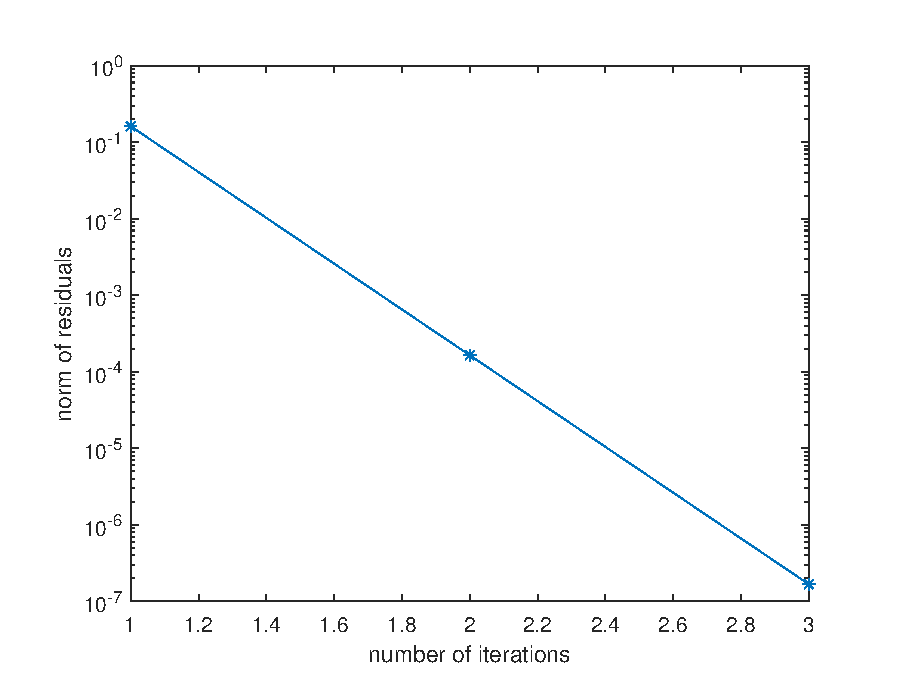
\includegraphics[width=8cm]{Pictures/F421_3.eps}
	\caption{reduction of residuals \\for V-cycle, full-weighting and linear interpolation\\ $n = 512$}
\end{figure}\\
\noindent \emph{Reduction rate of residuals = 0.0010209}\\
\emph{Max\_norm of error vector is 3.13641e-06}\\\\
$n=1024$: (Read 'Output/test421\_1024' for details)
\begin{figure}[!htp]   
	\centering
	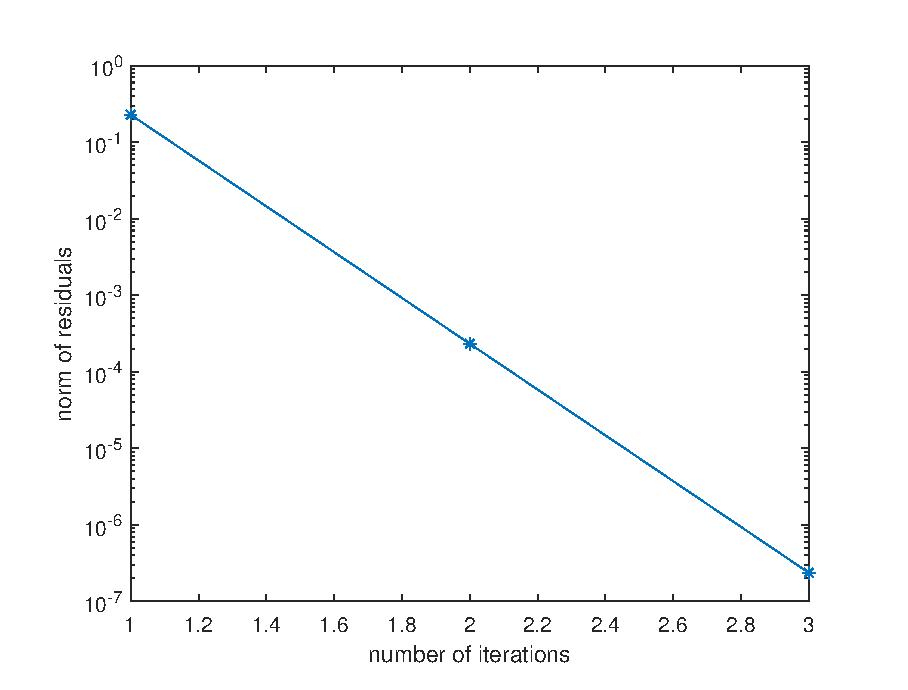
\includegraphics[width=8cm]{Pictures/F421_4.eps}
	\caption{reduction of residuals \\for V-cycle, full-weighting and linear interpolation\\ $n = 1024$}
\end{figure}\\
\noindent \emph{Reduction rate of residuals = 0.0010202}\\
\emph{Max\_norm of error vector is 7.83305e-07}\\\\
Then we have
\begin{table}[!htp]
	\centering
	\begin{tabular}{|c|c|c|}
		\hline	
		n & reduction rate of residuals &max-norm of err  \\
		\hline		
		128 &0.0010379& $5.01998\times 10^{-5}$ \\
		\hline		
		256 &0.0010243& $1.25489\times 10^{-5}$ \\
		\hline		
		512 &0.0010209& $3.13641\times 10^{-6}$ \\
		\hline		
		1024 &0.0010202& $7.83305\times 10^{-7}$ \\
		\hline
	\end{tabular}
	\caption{reduction rate of residuals and maximum norms of error vectors \\for V-cycle, full-weighting and linear interpolation}
\end{table}\\
\newpage
\noindent By simple calculation, we get that the convergence order in this case is 2.00065.
\subsubsection{Full-weighting and quadratic interpolation}
Except for restriction operators and interpolation operators, the inputfile is the same as the previous section. To avoid meaningless repetition, we show results only. More details can be obtained by reading corresponding output files.\\
Use command \textbf{"make test422"} to get results. 
\begin{table}[!htp]
	\centering
	\begin{tabular}{|c|c|c|}
		\hline	
		n & reduction rate of residuals & max-norm of err  \\
		\hline		
		128 &0.0043018 & $5.02007\times 10^{-5}$ \\
		\hline		
		256 &0.0045142 & $1.25497\times 10^{-5}$ \\
		\hline		
		512 &0.0048089 & $3.13722\times 10^{-6}$ \\
		\hline		
		1024 &0.0051308 & $7.8412\times 10^{-7}$ \\
		\hline
	\end{tabular}
	\caption{reduction rate of residuals and maximum norms of error vectors \\for V-cycle, full-weighting and quadratic interpolation}
\end{table}\\
The convergence order in this case is 2.00016.
\subsubsection{Injection and linear interpolation}
Show results only.Use command \textbf{"make test423"} to get results. \\
\begin{table}[!htp]
	\centering
	\begin{tabular}{|c|c|c|}
		\hline	
		n &reduction rate of residuals & max-norm of err \\
		\hline		
		128 &No data& $5.02009\times 10^{-5}$ \\
		\hline		
		256 &No data& $1.25499\times 10^{-5}$ \\
		\hline		
		512 &No data& $3.13747\times 10^{-6}$ \\
		\hline		
		1024 &No data& $7.84366\times 10^{-7}$ \\
		\hline
	\end{tabular}
	\caption{reduction rate of residuals and maximum norms of error vectors \\for V-cycle, injection and linear interpolation}
\end{table}\\
\newpage
\noindent The convergence order in this case is 2.00001.
\subsubsection{Injection and quadratic interpolation}
Show results only.Use command \textbf{"make test424"} to get results. \\
\begin{table}[!htp]
	\centering
	\begin{tabular}{|c|c|c|}
		\hline	
		n &reduction rate of residuals & max-norm of err \\
		\hline		
		128 &0.0033247& $5.02008\times 10^{-5}$ \\
		\hline		
		256 &0.0035345& $1.25499\times 10^{-5}$ \\
		\hline		
		512 &0.0037725& $3.13739\times 10^{-6}$ \\
		\hline		
		1024 &0.0039962& $7.84292\times 10^{-7}$ \\
		\hline
	\end{tabular}
	\caption{reduction rate of residuals and maximum norms of error vectors \\for V-cycle, injection and quadratic interpolation}
\end{table}\\
The convergence order in this case is 2.00006.
\subsection{Analysis of full multigrid cycle}
In this part, we will test the full multigrid cycle solver for all combinations of restriction operators and interpolation operators with $n$ = 128,256,512,1024 for homogeneous case. We will report the maximum norm of the error vector and the corresponding convergence rates.
\subsubsection{Full-weighting and linear interpolation}
Similar to the case of V-cycle, the input file is as follows:
\setlength{\tabcolsep}{1mm}{
	\begin{table}[!htp]
		\footnotesize
		\centering
		\begin{tabular}{|c|c|c|c|}
			\hline	
			Index&boundary&restriction&interpolation\\
			\hline		
			1&homogeneous&full\_weighting&linear\\	
			\hline		
			2& homogeneous&full\_weighting&linear\\	
			\hline		
			3& homogeneous&full\_weighting&linear\\
			\hline		
			4& homogeneous&full\_weighting&linear\\
			\hline \hline
			cycles&criteria\_type&criteria& initial\_type\\
			\hline
			fm\_cycle & 1 &1e-8 & 0 \\
			\hline
			fm\_cycle & 1 &1e-8 & 0 \\
			\hline
			fm\_cycle & 1 &1e-8 & 0 \\
			\hline
			fm\_cycle & 1 &1e-8 & 0 \\
			\hline
			\hline
			n & analysis &&\\
			\hline
			128 & 1 &&\\
			\hline
			256& 1 &&\\
			\hline
			512& 1 &&\\
			\hline
			1024& 1 &&\\
			\hline
		\end{tabular}
		\caption{Input test4-3-1}
\end{table}}
\newpage
\noindent Use command \textbf{"make test431"} to get results. 
\begin{table}[!htp]
	\centering
	\begin{tabular}{|c|c|}
		\hline	
		n  & max-norm of err \\
		\hline		
		128 & $5.02009\times 10^{-5}$ \\
		\hline		
		256 & $1.25464\times 10^{-5}$ \\
		\hline		
		512 & $3.13654\times 10^{-6}$ \\
		\hline		
		1024 & $7.8413\times 10^{-7}$ \\
		\hline
	\end{tabular}
	\caption{maximum norms of error vectors \\for full multigrid cycle, full-weighting and linear interpolation}
\end{table}\\
The convergence order in this case is 2.00016.
\subsubsection{Full-weighting and quadratic interpolation}
Except for restriction operators and interpolation operators, the inputfile is the same as the previous section. Similarly, we show results directly: (Use command \textbf{"make test432"} to get results.)
\newpage
\begin{table}[!htp]
	\centering
	\begin{tabular}{|c|c|}
		\hline	
		n  & max-norm of err \\
		\hline		
		128 & $5.02008\times 10^{-5}$ \\
		\hline		
		256 & $1.25499\times 10^{-5}$ \\
		\hline		
		512 & $3.13746\times 10^{-6}$ \\
		\hline		
		1024 & $7.84364\times 10^{-7}$ \\
		\hline
	\end{tabular}
	\caption{maximum norms of error vectors \\for full multigrid cycle, full-weighting and quadratic interpolation}
\end{table}
\balance
\noindent The convergence order in this case is 2.00001.
\subsubsection{Injection and linear interpolation}
Show results directly: (Use command \textbf{"make test433"} to get results.)
\begin{table}[!htp]
	\centering
	\begin{tabular}{|c|c|}
		\hline	
		n  & max-norm of err \\
		\hline		
		128 & $5.02009\times 10^{-5}$ \\
		\hline		
		256 & $1.25499\times 10^{-5}$ \\
		\hline		
		512 & $3.13747\times 10^{-6}$ \\
		\hline		
		1024 & $7.84367\times 10^{-7}$ \\
		\hline
	\end{tabular}
	\caption{maximum norms of error vectors \\for full multigrid cycle, injection and linear interpolation}
\end{table}\\
The convergence order in this case is 2.00001.
\subsubsection{Injection and quadratic interpolation}
Show results directly: (Use command \textbf{"make test434"} to get results.)
\begin{table}[!htp]
	\centering
	\begin{tabular}{|c|c|}
		\hline	
		n  & max-norm of err \\
		\hline		
		128 & $5.02009\times 10^{-5}$ \\
		\hline		
		256 & $1.25499\times 10^{-5}$ \\
		\hline		
		512 & $3.13747\times 10^{-6}$ \\
		\hline		
		1024 & $7.82266\times 10^{-7}$ \\
		\hline
	\end{tabular}
	\caption{maximum norms of error vectors \\for full multigrid cycle, injection and quadratic interpolation}
\end{table}\\
The convergence order in this case is 2.0013.
\end{document}
